O acionamento de um HSM pode ser realizado de diferentes formas para uma mesma configuração construtiva, sendo que cada forma proporciona vantagens diferentes. As principais característica que norteiam o tipo acionamento  é o número de  fases e o número de bobinas na máquina.

\subsection{Motores de Passo Unipolar e Bipolar}

Segundo BRITES\cite{PETele}, ao se acionar um motor de passo se deve estar atento a dois ponto importantes; primeiro que geralmente motores de passo possuem duas fases, devido principalmente a padronização dos dispositivos drives necessários para o acionamento, e segundo  que existem dois tipos de acionamento de polos; o acionamento unipolar e o bipolar.  

Nos motores de passo unipolar há dois enrolamentos por fase, que possuem um contato em comum, conhecido como \emph{center-tape}. Tal contato em comum pode ser usado para se colocar outras bobinas em paralelo, aumentando o numero de bobinas ativadas por passo. Porém a principal função do \emph{center-tape} é servir de ponto de alimentação do motor, de modo que para controlar a corrente pelas espiras se faz necessário penas aterrar um ou os dois terminas. A figura \ref{fig:MotorDePassoUnipolar} apresenta o diagrama de um motor de passo unipolar. 

\begin{figure}[H]
	\centering
	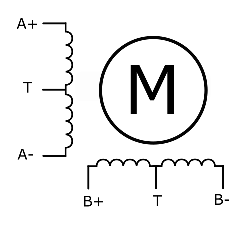
\includegraphics[width = 0.3 \columnwidth]{images/MotorDePassoUnipolar.eps}
	\caption{Motor de Passo Unipolar}
	\label{fig:MotorDePassoUnipolar}
\end{figure} 

Em relação aos terminas \emph{center-tape}, ou T como mostrado na figura \ref{fig:MotorDePassoUnipolar}, existem algumas variações de ligação onde se interliga os terminas T de modo a ficar disponível apenas 5 terminais na máquina, ou ainda onde se usa inúmeras fases todas com os terminais T curto-circuitados.   

Os motores bipolares basicamente não possuem o \emph{center-tape}, logo há apenas uma bobina por fase.  Logo para controlar a corrente pelas espiras se faz necessário o uso de circuitos mais complexos que possam inverter a alimentação das bobinas. A grande vantagem deste tipo de motor é o maior torque em relação ao motor unipolar. A figura \ref{fig:MotorDePassoBipolar} apresenta o diagrama de um motor de passo bipolar.

\begin{figure}[H]
	\centering
	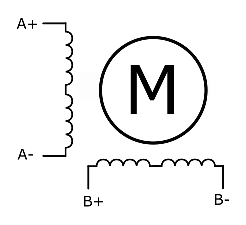
\includegraphics[width = 0.3\columnwidth]{images/MotorDePassoBipolar.eps}
	\caption{Motor de Passo Bipolar}
	\label{fig:MotorDePassoBipolar}
\end{figure}


\subsection{Modos de Acionamento} 

O acionamento de um motor de passo é realizado através da energização uma certa quantidade de bobinas de forma sequencial e repetida de acordo com o tipo de passo a se realizar. Existem três tipos de acionamento de bobinas para motores unipolares, e apenas um tipo de acionamento para motores bipolares. Cada tipo de acionamento requer uma configuração diferente de ligação entre bobinas.

A tabela \ref{Table:AcionamentoUnipolar} apresenta os três tipos de acionamento para motores unipolares. É importante salientar aqui que  para qualquer motor Unipolar independente do numero de fases se faz necessário, para qualquer tipo de acionamento apresentado, ter acesso a dois terminais cada fase e a apenas um terminal para o \emph{center-tape}, sendo este a alimentação do motor. Para inverter o sentido de giro do rotor seria necessário apenas inverter a alimentação no \emph{center-tape}, simplificando assim o circuito drive. 

\begin{table}[H]
	\centering
	\caption{Acionamento Para Motores Unipolares}
	\label{Table:AcionamentoUnipolar}
	\begin{tabular}{|cccc|}
		\hline
		\multicolumn{4}{|c|}{Wave Drive}  \\
		\hline
		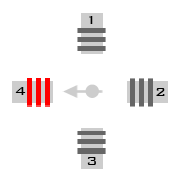
\includegraphics[width = 0.15\columnwidth]{Images/AcionamentoDoHSM/Unipolar/WaveDrive/WaveDriveI.png}& 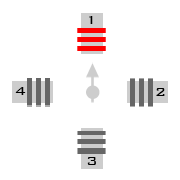
\includegraphics[width = 0.15\columnwidth]{Images/AcionamentoDoHSM/Unipolar/WaveDrive/WaveDriveII.png} & 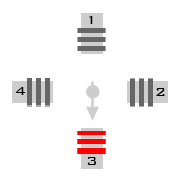
\includegraphics[width = 0.15\columnwidth]{Images/AcionamentoDoHSM/Unipolar/WaveDrive/WaveDriveIII.png} & 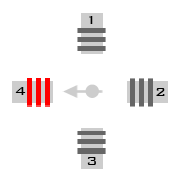
\includegraphics[width = 0.15\columnwidth]{Images/AcionamentoDoHSM/Unipolar/WaveDrive/WaveDriveIV.png} \\
		\hline
		\multicolumn{4}{|c|}{Full Drive}  \\
		\hline
		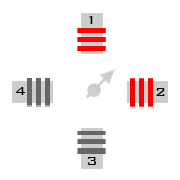
\includegraphics[width = 0.15\columnwidth]{Images/AcionamentoDoHSM/Unipolar/FullDrive/FullDriveI.png} & 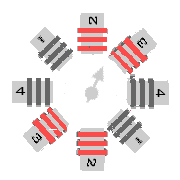
\includegraphics[width = 0.15\columnwidth]{Images/AcionamentoDoHSM/Unipolar/FullDrive/FullDriveII.png}   & 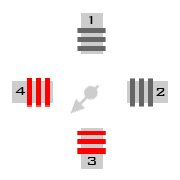
\includegraphics[width = 0.15\columnwidth]{Images/AcionamentoDoHSM/Unipolar/FullDrive/FullDriveIII.png}   &  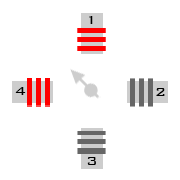
\includegraphics[width = 0.15\columnwidth]{Images/AcionamentoDoHSM/Unipolar/FullDrive/FullDriveIV.png}  \\
		\hline
		\multicolumn{4}{|c|}{Half Drive} \\
		\hline
		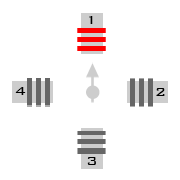
\includegraphics[width = 0.15\columnwidth]{Images/AcionamentoDoHSM/Unipolar/HalfDrive/HalfDriveI.png} & 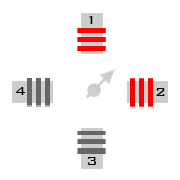
\includegraphics[width = 0.15\columnwidth]{Images/AcionamentoDoHSM/Unipolar/HalfDrive/HalfDriveII.png} & 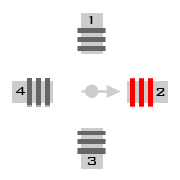
\includegraphics[width = 0.15\columnwidth]{Images/AcionamentoDoHSM/Unipolar/HalfDrive/HalfDriveIII.png} & 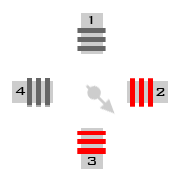
\includegraphics[width = 0.15\columnwidth]{Images/AcionamentoDoHSM/Unipolar/HalfDrive/HalfDriveIV.png} \\
		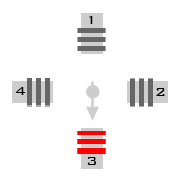
\includegraphics[width = 0.15\columnwidth]{Images/AcionamentoDoHSM/Unipolar/HalfDrive/HalfDriveV.png} & 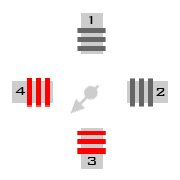
\includegraphics[width = 0.15\columnwidth]{Images/AcionamentoDoHSM/Unipolar/HalfDrive/HalfDriveVI.png} & 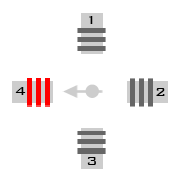
\includegraphics[width = 0.15\columnwidth]{Images/AcionamentoDoHSM/Unipolar/HalfDrive/HalfDriveVII.png} & 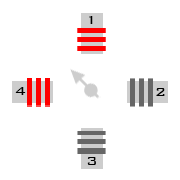
\includegraphics[width = 0.15\columnwidth]{Images/AcionamentoDoHSM/Unipolar/HalfDrive/HalfDriveVIII.png} \\			
		\hline
	\end{tabular}
\end{table}


A tabela \ref{Table:AcionamentoBipolar} apresenta apenas o método de acionamento \emph{Wave Drive}. Neste método de acionamento se faz necessário apenas 2 terminais para cada fase. Porém a grande desvantagem deste método de acionamento é a necessidade de um circuito capaz de inverter a corrente em cada uma das bobinas, logo resultando em um circuito driver mais complexo. 

\begin{table}[H]
	\centering
	\caption{Acionamento Para Motores Bipolares}
	\label{Table:AcionamentoBipolar}
	\begin{tabular}{|cccc|}
		\hline
		\multicolumn{4}{|c|}{Wave Drive Bipolar}  \\
		\hline
		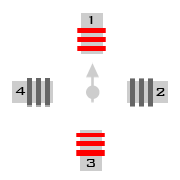
\includegraphics[width = 0.15\columnwidth]{Images/AcionamentoDoHSM/Bipolar/WaveDrive/WaveDriveI.png} & 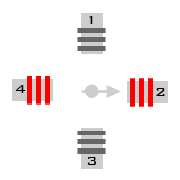
\includegraphics[width = 0.15\columnwidth]{Images/AcionamentoDoHSM/Bipolar/WaveDrive/WaveDriveII.png} & 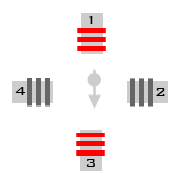
\includegraphics[width = 0.15\columnwidth]{Images/AcionamentoDoHSM/Bipolar/WaveDrive/WaveDriveIII.png} & 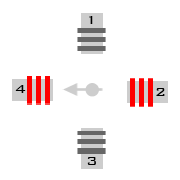
\includegraphics[width = 0.15\columnwidth]{Images/AcionamentoDoHSM/Bipolar/WaveDrive/WaveDriveIV.png} \\
		\hline
	\end{tabular}
\end{table} 
